%%%%%%%%%%%%%%%%%%%%%%%%%%%%%%%%%%%%%%%%%%%%%%%%%%%%%%%%%%%%%%%%%%%%%%%%%%%%%%%
% Chapter 3 - Spatially-Targeted Photothrombotic Stroke
%%%%%%%%%%%%%%%%%%%%%%%%%%%%%%%%%%%%%%%%%%%%%%%%%%%%%%%%%%%%%%%%%%%%%%%%%%%%%%%

\chapter{Spatially-Targeted Photothrombotic Stroke}

\blindtext


%%%%%%%%%%%%%%%%%%%%%%%%%%%%%%%%%%%%%%%%%%%%%%%%%%%%%%%%%%%%%%%%%%%%%%%%%%%%%%%
% Section 3.1 - Instrumentation Modifications
%%%%%%%%%%%%%%%%%%%%%%%%%%%%%%%%%%%%%%%%%%%%%%%%%%%%%%%%%%%%%%%%%%%%%%%%%%%%%%%
\section{Instrumentation Modifications}

The system was modified (Figure \ref{fig:systemschematic_2}) to perform photothrombotic stroke with the addition of a 532 nm laser (200 mW, AixiZ). The packaged diode laser has a 2 mm collimated output that operates at a fixed current with convection cooling. A neutral density filter (OD 1.0, NE10A-A, Thorlabs, Inc.) was used to attenuate the laser intensity by an order of magnitude. A longpass dichroic beamsplitter (490 nm cutoff, DMLP490, Thorlabs, Inc.) was used to coalign the 532 nm laser with the other two lasers for coupling into the fiber optic patch cord. The green light can then be patterned by the DMD for targeted photothrombosis. \ce{pO2} measurements can be acquired simultaneously during photothrombosis induction because of the system's spectral separation, but are limited to only the targeted region.

% Figure - System Schematic (Ver. 2)
\begin{figure}
    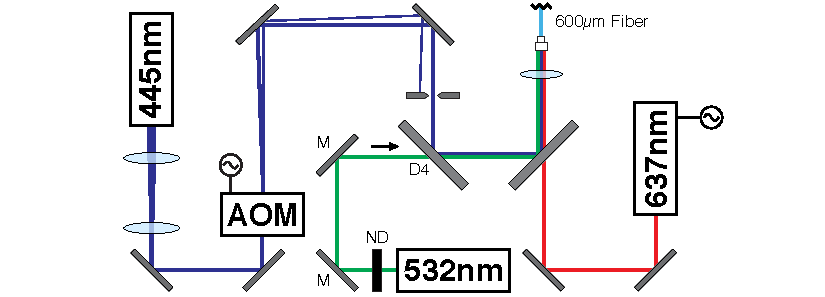
\includegraphics{figures/chapter_3/systemschematic_2.pdf}
    \caption {
        \label{fig:systemschematic_2}
        The optical system was modified with the addition of a 532 nm laser coupled into the fiber optic patch cord for DMD-targeted photothrombosis.
    }
\end{figure}



%%%%%%%%%%%%%%%%%%%%%%%%%%%%%%%%%%%%%%%%%%%%%%%%%%%%%%%%%%%%%%%%%%%%%%%%%%%%%%%
% Section 3.2 - Targeted Photothrombosis Induction
%%%%%%%%%%%%%%%%%%%%%%%%%%%%%%%%%%%%%%%%%%%%%%%%%%%%%%%%%%%%%%%%%%%%%%%%%%%%%%%
\section{Targeted Photothrombosis Induction}

Targeted photothrombosis was demonstrated \textit{in vivo} using anesthetized (1.5\% isoflurane in medical air) mice with permanent cranial window implants. Rose bengal was administered intravenously via retro-orbital injection (50 $\mu$L, 15 mg/mL) and the subject was immediately exposed to DMD-patterned green light for 5-10 minutes. Descending arterioles were the primary targets because they serve as bottlenecks in the cortical oxygen supply \cite{Nishimura:2007hk}. Target vessels were identified based on vascular orientation and \textit{a posteriori} knowledge. \ce{pO2} measurements were limited when performing photothrombosis to only the region being targeted for occlusion and were acquired continuously with 2500 decays being averaged per record. LSCI was used to monitor clot formation within the targeted area and control the progression of the occlusion.

%%%%%%%%%%%%%%%%%%%%%%%%%%%%%%%%%%%%%%%%%%%%%%%%%%%%%%%%%%%%%%%%%%%%%%%%%%%%%%%
\subsection{Photothrombosis Hemodynamics}

\blindtext



%%%%%%%%%%%%%%%%%%%%%%%%%%%%%%%%%%%%%%%%%%%%%%%%%%%%%%%%%%%%%%%%%%%%%%%%%%%%%%%
% Section 3.3 - Targeted Photothrombosis Induction
%%%%%%%%%%%%%%%%%%%%%%%%%%%%%%%%%%%%%%%%%%%%%%%%%%%%%%%%%%%%%%%%%%%%%%%%%%%%%%%
\section{Targeted Photothrombosis Induction}

\blindtext



%%%%%%%%%%%%%%%%%%%%%%%%%%%%%%%%%%%%%%%%%%%%%%%%%%%%%%%%%%%%%%%%%%%%%%%%%%%%%%%
% Section 3.4 - Discussion
%%%%%%%%%%%%%%%%%%%%%%%%%%%%%%%%%%%%%%%%%%%%%%%%%%%%%%%%%%%%%%%%%%%%%%%%%%%%%%%
\section{Discussion}

\blindtext



%%%%%%%%%%%%%%%%%%%%%%%%%%%%%%%%%%%%%%%%%%%%%%%%%%%%%%%%%%%%%%%%%%%%%%%%%%%%%%%
% END Chapter 3
%%%%%%%%%%%%%%%%%%%%%%%%%%%%%%%%%%%%%%%%%%%%%%%%%%%%%%%%%%%%%%%%%%%%%%%%%%%%%%%
